\documentclass{comjnl}

\usepackage{amsmath}
\usepackage{blindtext}
\usepackage{braket}
\usepackage{multicol}
\usepackage{float}
%% These two lines are needed to get the correct paper size
%% in TeX Live 2016
\let\pdfpageheight\paperheight
\let\pdfpagewidth\paperwidth

%\copyrightyear{2009} \vol{00} \issue{0} \DOI{000}

\begin{document}

\title[title]{title}
\author{jefferson deyvis}
\affiliation{Intelligent Systems and Networks Group, Department of
Electrical and Electronic Engineering, Imperial College, London
SW7 2BT, UK} \email{kumaara.velan@imperial.ac.uk}

\shortauthors{K. Velan}
 
\received{00 January 2009}
\revised{00 Month 2009}


%\category{C.2}{Computer Communication Networks}{Computer Networks}
%\category{C.4}{Performance of Systems}{Analytical Models}
%\category{G.3}{Stochastic Processes}{Queueing Systems}
%\terms{Internet Technologies, E-Commerce}
\keywords{Automated Auctions; Analytical Models; Autonomic
Systems; Internet Technologies; E-Commerce; Queueing Systems}


\begin{abstract}

\blindtext

\end{abstract}

\maketitle

\section{Introduction}

\blindtext

\section{The model} \label{Model}

\noindent Our model consists of a one-dimensional chain of atoms, built from a font, $\ket{s}$, a channel with $N$ atoms and a receiver $\ket{R}$. The full channel contains $N+2$ atoms.
\begin{figure}[ht]
  \centering
  
\includegraphics[width= 22em]{fonte.png}
  \caption{Chain of $N$ atoms with a font and receiver}
\end{figure}

\noindent In our model, the Hamiltonian is given by:


\begin{equation}
    \hat{H} = \ket{s}\bra{s}\varepsilon_s + g(\ket{s}\bra{2} + \ket{N+1}\bra{R})+ \ket{R}\bra{R}\varepsilon_R + \hat{H}_c
\end{equation}

\noindent where $g$ is the \textit{hopping Amplitude} between the atoms $\ket{s}$ and $\ket{2}$ and between $\ket{N+1}$ and $\ket{R}$, $\hat{H}_c$ is given by:

\begin{equation}
    \hat{H}_c = \sum_{i=2}^{N+1} \ket{i}\bra{i}\varepsilon_i + T \sum_{i=2}^{N+1}  \ket{i+1}\bra{i} + c.c
\end{equation}

\noindent where $T$ is the \textit{hopping Amplitude} in chain atoms, and the set $\{\varepsilon_i\}$ is a series with long-range correlated disorder generated from:

\begin{equation}\label{lorentzian}
    y_i = \sum_{j=1}^N z_j(1+|i-j|/A)^2
\end{equation}
where $z_j$ is a randon number belong to the range $[-1,1]$, and $A$ is an adjustment parameter, so $\varepsilon_i$ is constructed as follows:

\begin{equation}
    \varepsilon_i =(y_i - \bar{y_i})\sqrt{\bar{y_i^2} - \bar{y_i}^2}
\end{equation}

\noindent Let's write the Hamiltonian in its matrix form:

\begin{equation}
\begin{pmatrix}
    \varepsilon_s  & g & 0 & 0 & \dots & 0 & 0\\
    g & \varepsilon_2  & T & 0 & \dots & 0 & 0\\
    0 & T & \varepsilon_3  & T & \dots & 0 & 0\\
    0 & 0 & T & \varepsilon_4 & \dots  & 0 & 0\\
    \vdots & \vdots & \vdots  & \vdots & \ddots & T & 0\\
    0 & 0 & 0 & 0 & T & \varepsilon_{N+1} & g\\
    0 & 0 & 0 & 0 & 0 & g & \varepsilon_R\\
\end{pmatrix}
\end{equation}

\section{Results}  
\subsection{Autocorrelation}
The autocorrelation of the set $\{\varepsilon_i\}$ can be obtained by:

\begin{equation}
    C(r) = <\varepsilon_i\varepsilon_{i+r}>-<\varepsilon_i><\varepsilon_{i+r}>
\end{equation}

\noindent where $<\varepsilon_i\varepsilon_{i+r}>$ is given by:

\begin{equation*}
    <\varepsilon_i\varepsilon_{i+r}> = \frac{1}{N-r}\sum_{i=1}^{N-r}\varepsilon_i\varepsilon_{i+r} \quad
    <\varepsilon_{i}>=\sum_{i=1}^{N}\varepsilon_i
\end{equation*}

\begin{figure}[ht]
  \centering
  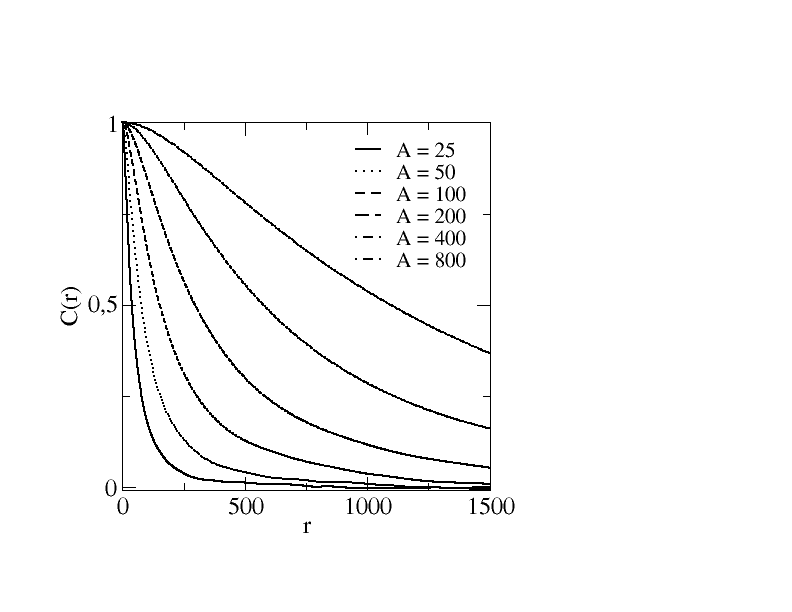
\includegraphics[width= \linewidth]{acr.png}
  \caption{series $\varepsilon_i$ autocorrelation by fitting equation (3) for different values of $A$}
\end{figure}

\subsection{Participation}
\noindent The diagonalization of Hamiltonian matrix provides the eigenstates $\ket{\Psi_i}$ and the eigenvalues $E_i$, and we can expand the eigenstates on the orbital basis ($\ket{\Psi_i} = \sum_{n=1}^N f_n^{(i)} \ket{n}$).The participation is a a
number that measures the degree of location of states. This measure is given by:

\begin{equation}
    \displaystyle{P = \frac{1}{\sum_j |f_n|^4}}
\end{equation}

\begin{figure}[ht]
  \centering
  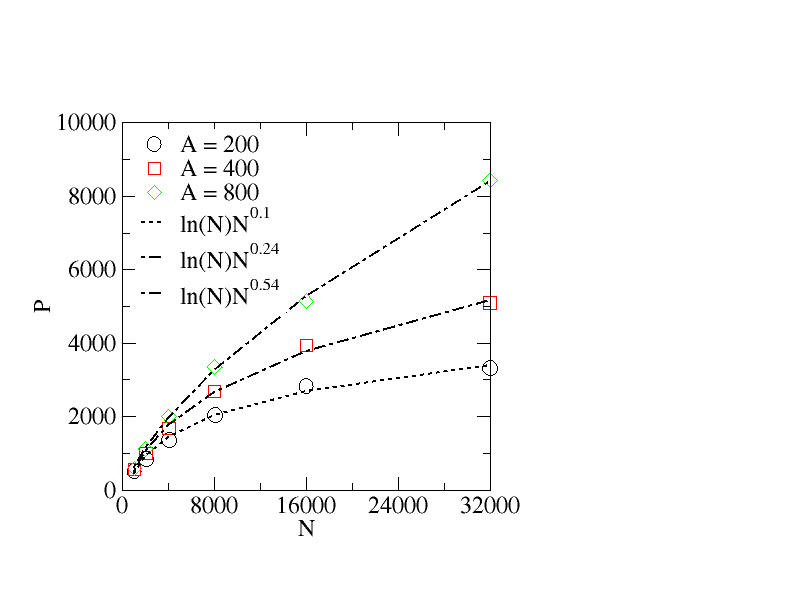
\includegraphics[width= \linewidth]{PN.png}
  \caption{maximum participation versus $N$ where each curve corresponds to a single value of $A$.}
\end{figure}

\begin{figure}[ht]
  \centering
  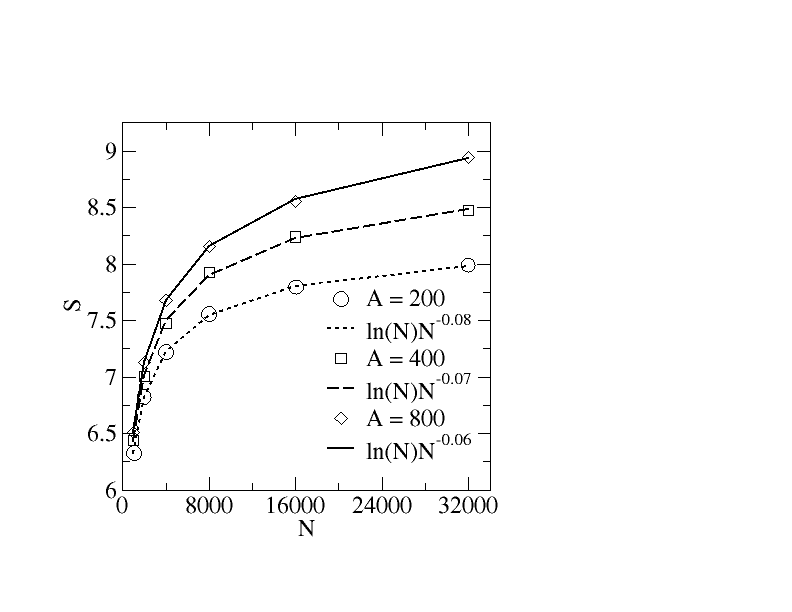
\includegraphics[width= \linewidth]{entropy.png}
  \caption{\textit{Shannon entropy} versus $N$ where each curve corresponds to a single value of $A$.}
\end{figure}

\begin{figure*}[!htbp]
  \centering
  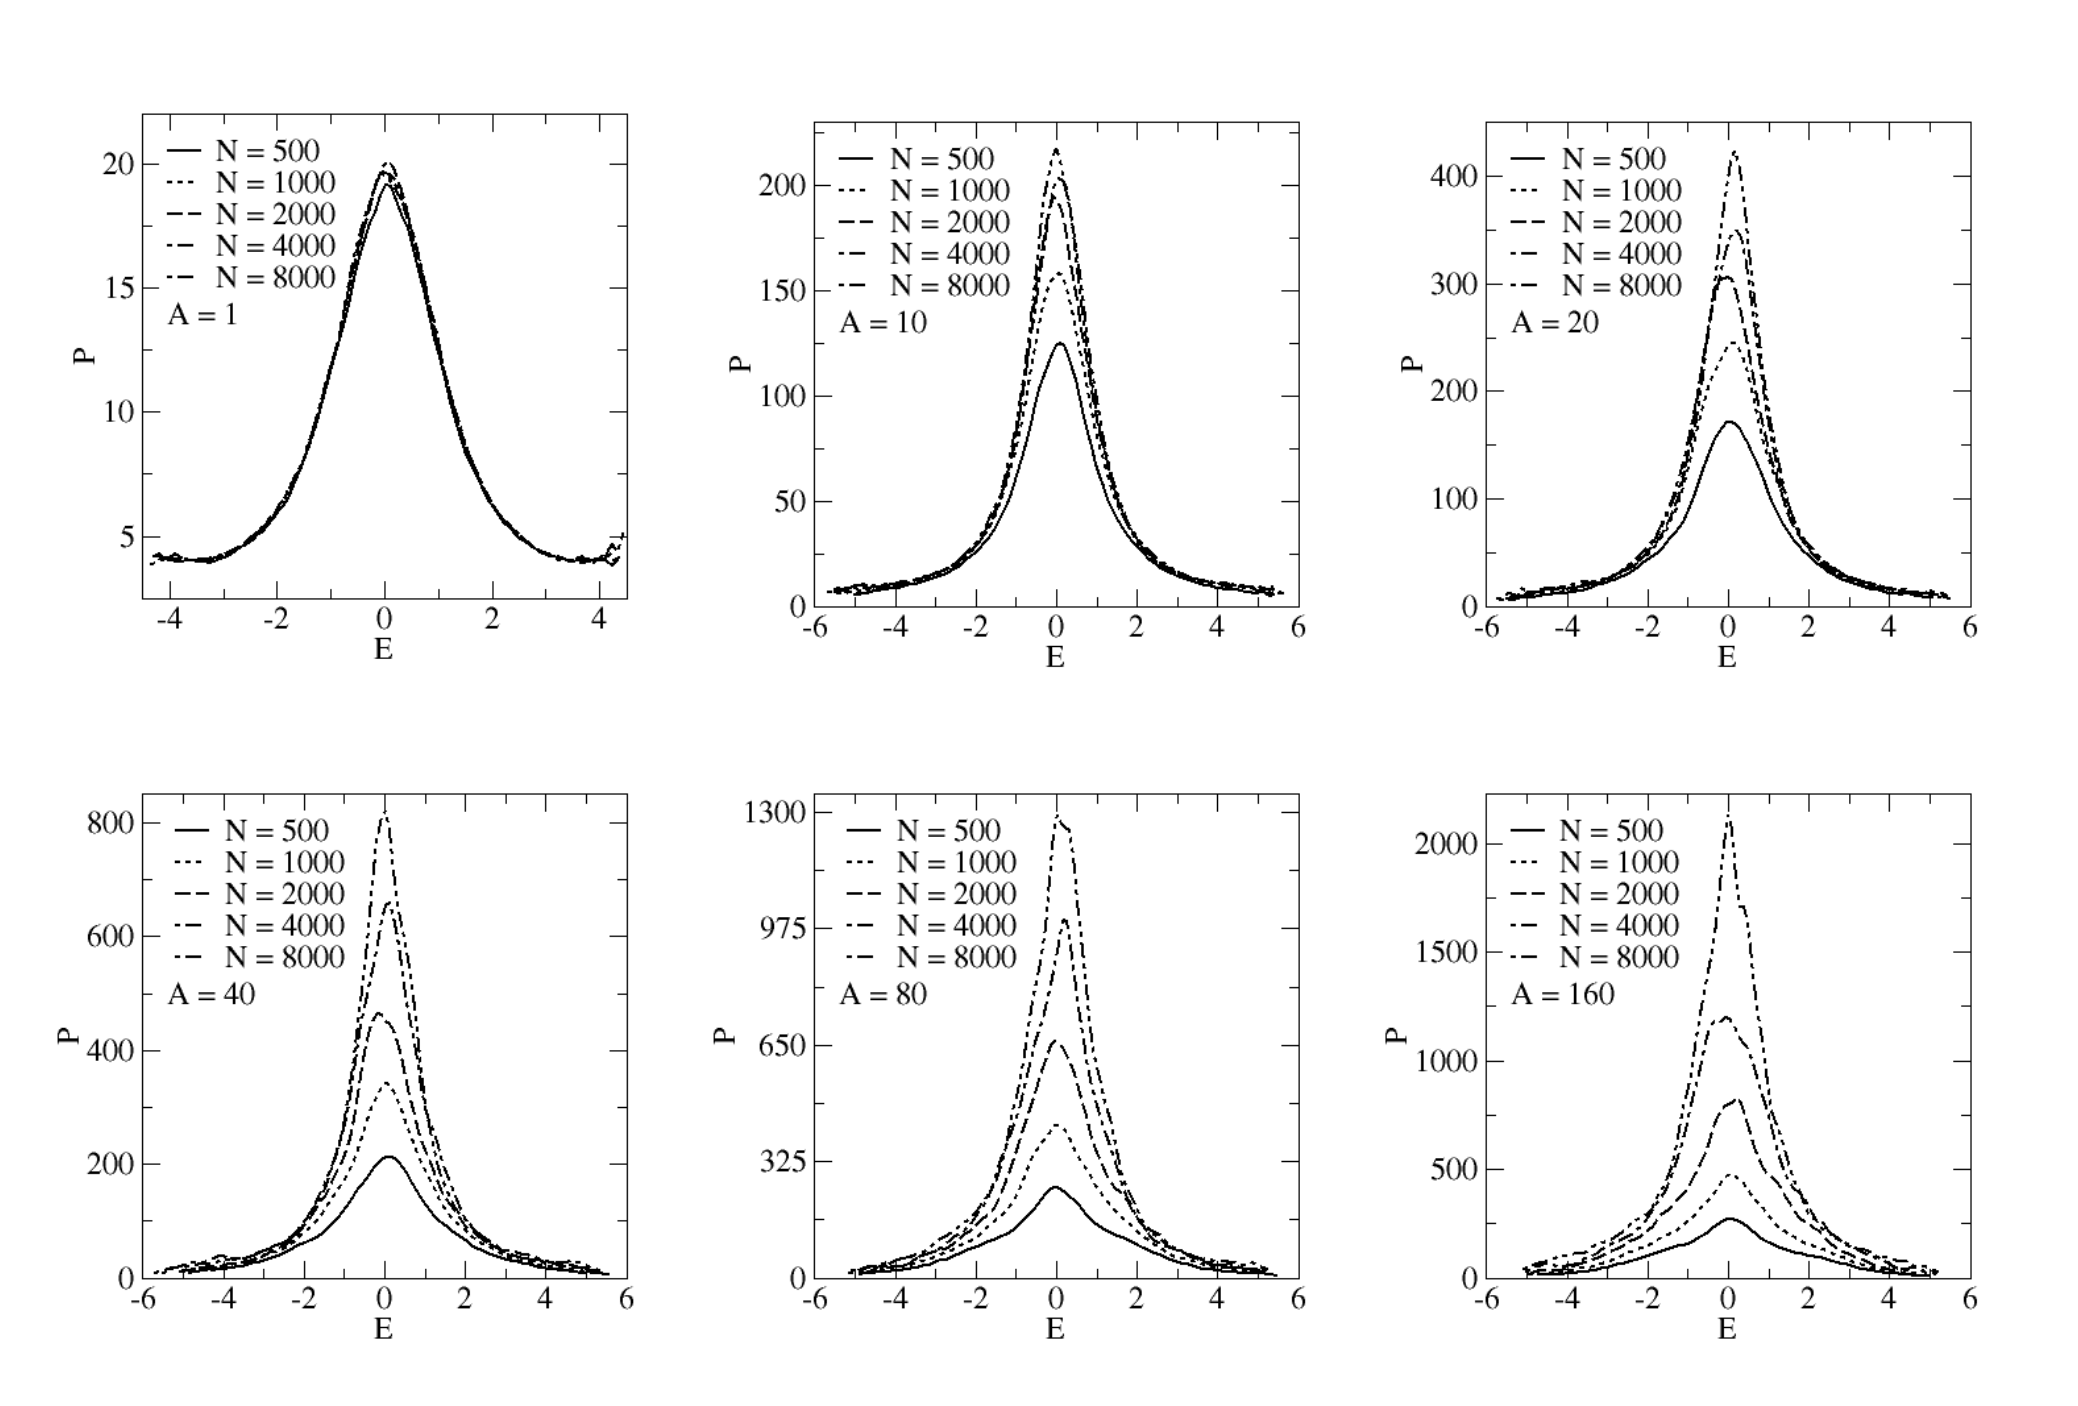
\includegraphics[width=\linewidth]{PE.png}
  \caption{maximum participation versus $E$ where each curve corresponds to a single value of $A$.}
\end{figure*}

\subsection{Fidelity}

\begin{figure}[ht]
  \centering
  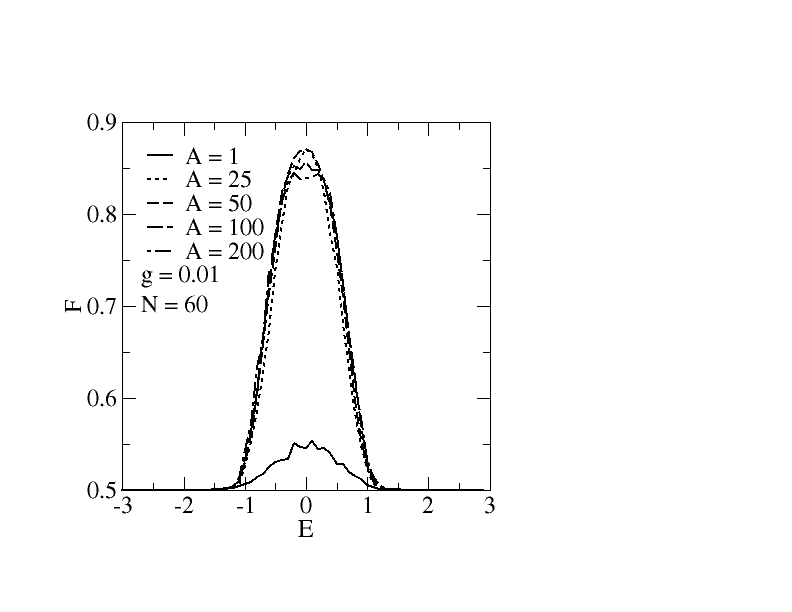
\includegraphics[width= \linewidth]{fidelidade.png}
  \caption{maximum Fidelity versus $\Omega$ where each curve corresponds to a single value of $A$, $N = 60$ and $g = 0.01$.}
\end{figure}

\begin{figure}[ht]
  \centering
  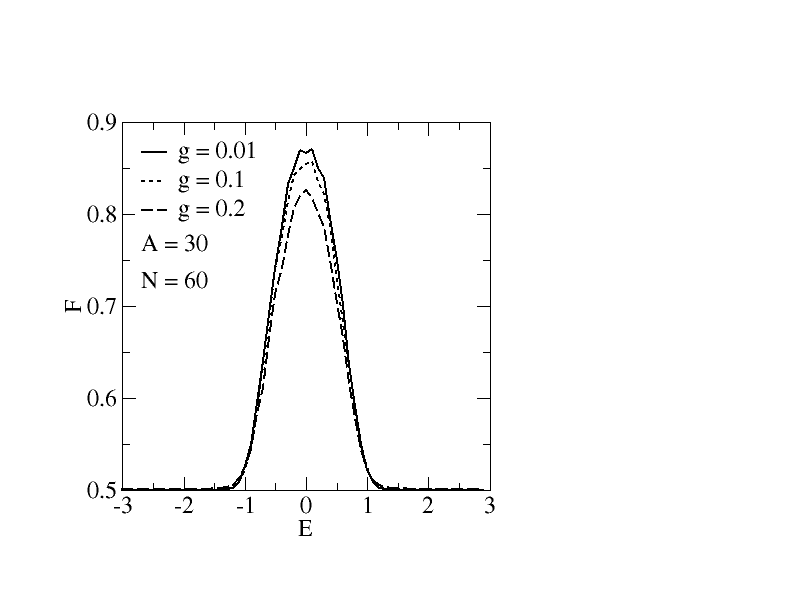
\includegraphics[width= \linewidth]{FgA30.png}
  \caption{maximum Fidelity versus $\Omega$ where each curve corresponds to a single value of $g$, $N = 60$ and $A = 30$.}
\end{figure}

\begin{figure}[ht]
  \centering
  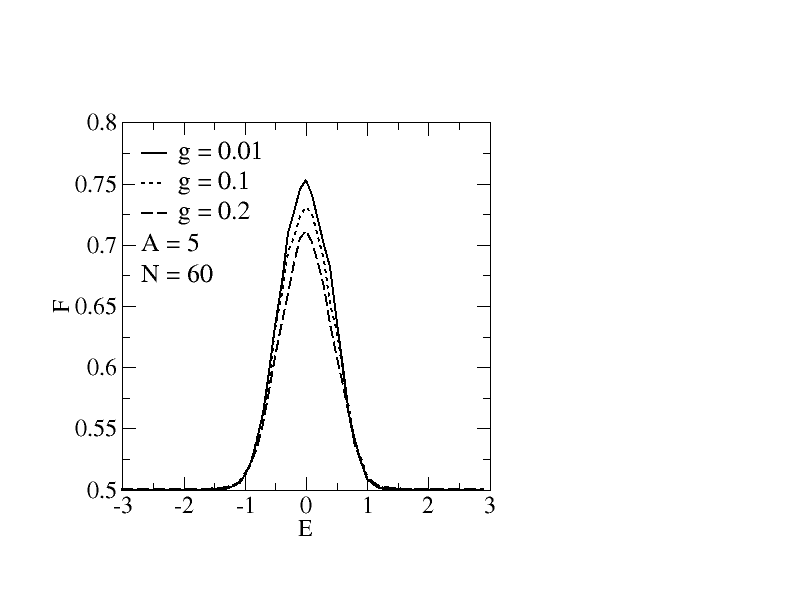
\includegraphics[width= \linewidth]{FgA5.png}
  \caption{maximum Fidelity versus $\Omega$ where each curve corresponds to a single value of $A$, $N = 60$ and $A = 5$.}
\end{figure}

\subsection{concurrence}

\begin{figure}[ht]
  \centering
  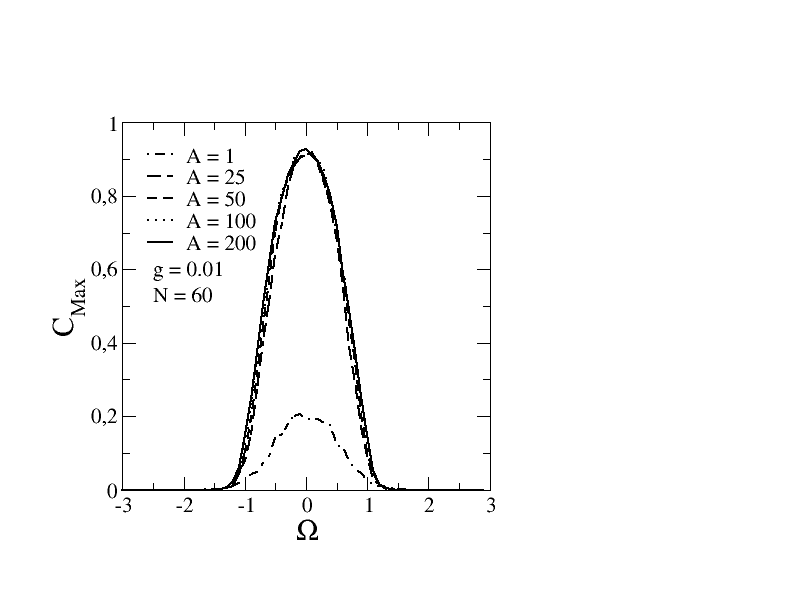
\includegraphics[width= \linewidth]{concorrencia.png}
  \caption{maximum concurrence versus $\Omega$ where each curve corresponds to a single value of $g$, $N = 60$ and $g = 0.01$.}
\end{figure}

\begin{figure}[ht]
  \centering
  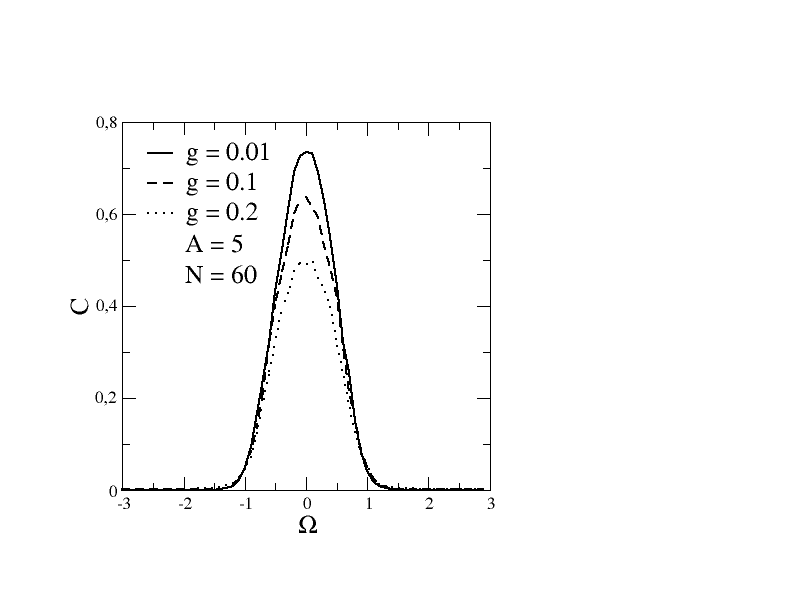
\includegraphics[width= \linewidth]{cga5.png}
  \caption{maximum concurrence versus $\Omega$ where each curve corresponds to a single value of $A$, $N = 60$ and $A = 5$.}
\end{figure}

\begin{figure}[ht]
  \centering
  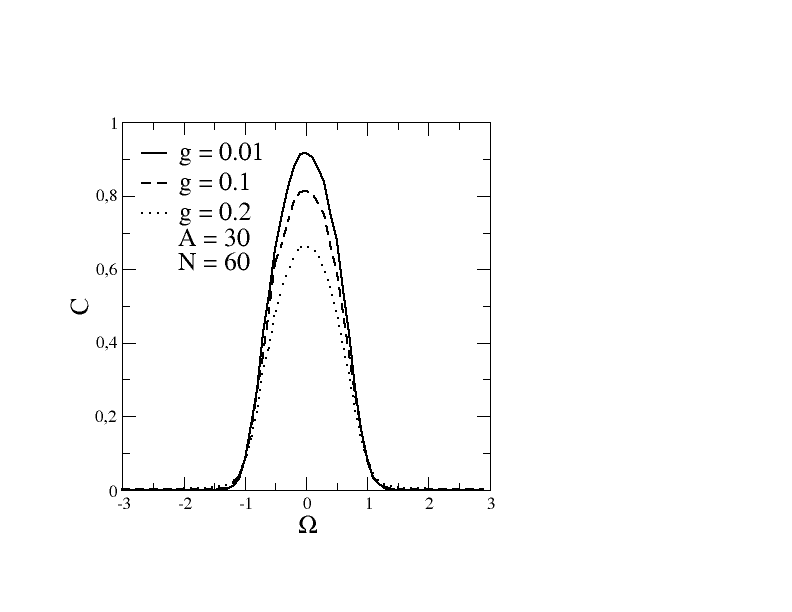
\includegraphics[width= \linewidth]{cga30.png}
  \caption{maximum concurrence versus $\Omega$ where each curve corresponds to a single value of $A$, $N = 60$ and $A = 30$.}
\end{figure}


\section{Conclusions} \label{Conclusions}


\bibliographystyle{compj}
\bibliography{ModellingBidders}


\end{document}